\documentclass[10pt]{beamer}
\usepackage{xeCJK}
\usepackage{graphicx}
\usepackage{booktabs}
\usepackage{listings}
\usepackage{multirow}
\usepackage{mathtools}
\usepackage{ulem}
\usefonttheme[onlymath]{serif}
\usetheme{metropolis}
\setbeamercolor{footnote mark}{fg=blue}% set footnote color in beamer
\setbeamerfont{footnote}{size=\tiny}
\begin{document}
	\title{浅谈求交互参数类交互问题}
	\date{\today}
	\author{雅礼中学~~胡昊}
	\maketitle
	
	\begin{frame}
		\frametitle{摘要}
		
		交互题正在逐渐成为当今OI的重要考点,它的考法包括求交互参数、博弈等考法。

		我的论文将介绍求交互参数类问题的考法,三种解决方案与优化方法。
	\end{frame}
	
	\begin{frame}
		\frametitle{交互参数类问题}
	
		如果把交互库看做是一个C++中的class$f$,交互参数是$x$,你的询问$y$,那么返回的就是$f(x,y)$,你的目的就是猜出这一个$x$。这个过程可以被下图描述:

		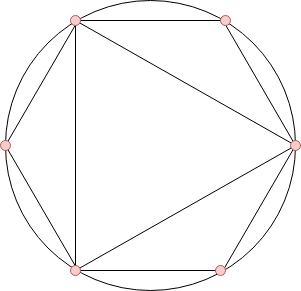
\includegraphics[width=0.7\textwidth]{1.png}

	\end{frame}
	
	\begin{frame}
		\frametitle{逐步增加方便利用的已知信息}
		在一道题的开始,可以认为已知信息为空,或者选定一个元素作为初始的已知信息,然后在后面的每一次操作中,目标都是将可以利用的已知信息变多。

		在某一道题中,你的目标是求出隐藏的一个序列,题目保证了可以通过前面的若干元素加以询问得到后面的元素,这样我们可以从序列的开头向后依次确定,便于利用的信息就是这个序列的一个前缀;但是如果你知道零散几个位置的值,并不方便利用,这就不是方便利用的信息。
		
		又比如说在另一道题中,你的目标是求出一个隐藏的无向图,我们可以找一个点作为初始连通块,然后不断通过询问扩大,在这里便于利用的信息就是你找到的一个点集的导出子图;但是如果你知道零散几条边,在后面的询问中不好利用,甚至会重复地求出,这就不是方便利用的信息。
	\end{frame}
	
	\begin{frame}
		\frametitle{图例}
	
		这个过程就像下图在黑色区域类加入红色点一样:

		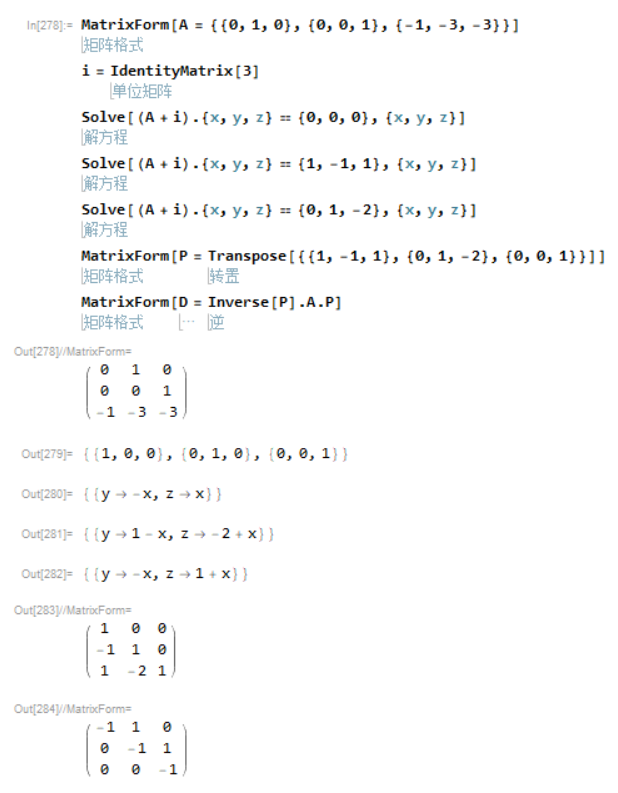
\includegraphics[width=0.7\textwidth]{3.png}
	\end{frame}
	
	\begin{frame}
		\frametitle{例题1:组合动作\footnote{International Olympiad in Informatics(IOI) 2018}}
	
		交互库有一个长度为$n$字符集大小为$4$的字符串$S$,你需要通过询问求出并输出这个字符串。每次可以询问一个长度小于$4n$的字符串$T$,会返回最大的$v$,使得$S$的长度为$v$的前缀是$T$的子串。特别的,$S$的第一个字符在$S$中仅出现一次。
	
		\onslide<2->
		
		如果我们知道了$S$的一个前缀$S_p$,那么如果询问$S_pa$返回True,那么$S_pa$是$S$的一个更长的前缀。于是,可以将$S_p$视为我们所说的便于利用的性质。

		先通过$2$次询问确定下第一位,然后用刚才的方法不断地得到$S$的前缀。

		题目的性质保证了它可以优化,但因为适用范围不广,就在这里简述了:通过一次询问$S_paS_pbaS_pbbS_pbc$就可以确定S的下一位,这样就是$n+O(1)$次询问了。

	\end{frame}
	
	\begin{frame}
		\frametitle{例题1改编}

		交互库有一个长度为$n$字符集大小为$2$的字符串$S$,你的目标是通过询问求出并输出它。你每次可以询问一个字符串,交互库会返回它是否是$S$的子串。
		
		\onslide<2->
		
		如果我们用和上题相同的方法,可以但也只能得到$S$的一个后缀(在$S$的后缀后面加0或1都会返回False,可以以此判断是否是$S$的后缀),我们可以通过在这个字符串前面添加元素,来得到整个串。
		
		套用上题的优化方法,但如果询问S'0返回False,就认为S'的下一位是1的话,可能会出现问题:此时是序列末尾。每隔$\sqrt n$次判断一下现在是否是序列末尾就可以做到$n+O(\sqrt n)$次询问内求解了。
		
	\end{frame}
	
	\begin{frame}
		\frametitle{例题2:自然公园\footnote{Japanese Olympiad in Informatics Spring Camp(JOISC) 2017}}
	
		交互库有一个无向图,你要求出并输出每一条边。你每次可以询问两个点和一个点集,会返回这两个点在这个点集的导出子图内是否处于同一连通块。

		\onslide<2->

		我们选定任意一个点作为初始点集,不断找到一个与当前点集相连的点(如果仅通过当前点集的点能到达点集内任意一点,就相邻),并找到连至点集内的所有边,将这个点加入点集。

		这个过程和之前展示的图例完全一致。

	\end{frame}
	
	\begin{frame}
		\frametitle{例题3:So Mean\footnote{codeforces 1299 E}}

		交互库有一个排列,保证第一个数小于$\dfrac n2$,你需要求出并输出这一个排列。每次可以询问若干位置,会返回这些位置上的数的平均值是否是整数。
		
		\onslide<2->
		
		通过观察发现,我们询问$\{l,l+1,l+2\dots,r\}-\{x\}$时,交互库返回的是$x$是否是$l$到$r$中的最大或最小值,我们就可以不断的找出未知位置中的最大与最小值。
		
	\end{frame}
	
	\begin{frame}
		\frametitle{例题4:即时战略\footnote{Winter Camp(WC) 2018}}

		交互库有一棵树,你需要求出并输出每一条边。每次可以询问$x,y$,交互库会返回$x,y$路径上距离$x$距离为$1$的点。
		
		\onslide<2->
		
		我们可以挑任意一个点为根,对于剩下每一个点都可以通过不断的询问找到根到它的路径,这样就可以还原出树的形态了。
	
	\end{frame}
	
	\begin{frame}
		\frametitle{优化}
	
		在很多题目中,最为朴素的算法是不足以通过的,我们需要找到优化的方案。

		要找到优化方案,要先对先前的算法有更深的理解,通过归纳总结,多数情况下我们使用的算法就是重复的执行下面两步:

		\begin{enumerate}
			\item 找到一个未知的元素。
			\item 找到这个元素与已知信息中元素的关系。
		\end{enumerate}

		很多时候,这两个步骤是可以优化的,和优化数据结构题类似,可以先找到复杂度的瓶颈,然后针对这一瓶颈套用常用的$\log$或者根号算法:分治、分块等。

	
	\end{frame}
	
	\begin{frame}
		\frametitle{例题2优化1}

		这道题中,第一步是找到与已知点集相邻的一个点,第二步是找到这个点已知点集的所有边。课件在这道题中,两个步骤都是复杂度的瓶颈。第一步的优化将在后文中展示,这里先介绍第二步的优化。
		
		不妨假设一个点为根,便于寻找点$u$和已知集合的关系。这里有一个引理:
		
		{\color[rgb]{0,0,0}{对于联通点集$S$,点$x,y,z$,满足$x,y\in S,z\not\in S$:若满足$S-\{x\}$是联通的,若$z$在仅经过$S$中的点能到达$y$,但在仅经过$S-\{x\}$中的点不能到$y$,则$x,z$有边直接相连。}}
		
		证明是:若$x$与$z$无直接边相连,考虑$z$到$y$的第一步$z\rightarrow r$,因为$S-\{x\}$联通,所以$r$可以在不经过$x$的情况下到达$y$,与假设矛盾。
		
		利用这一个引理,可以通过二分快速找到一条与$u$相连的边:任意找到一个已知点集的生成树,在它的先序遍历上二分即可,先序遍历的前缀一定组成连通块,与引理的要求相符。
	
	\end{frame}
	\begin{frame}
		\frametitle{例题3优化}
		
		在这一道题的解法中,并没有用上元素间的关系,仅仅是找到有集合中最大/最小这个性质的元素,所以可以认为第一步是复杂度的瓶颈,针对这个步骤,可以找到优化:
		
		在第一次询问后,可以将所有元素分为奇数和偶数(询问$1$和这个元素即可),就将数据规模变为了$\dfrac 12$;类似的,再根据$\bmod 4$分为四个部分,数据规模就变为了$\dfrac 14$……
		
		这样就不断让数据规模变为一半,复杂度满足递归式$T(n)=2T(\dfrac n2)+O(n)$,根据主定理有:$T(n)=O(n\log n)$。
		
	
	\end{frame}
	\begin{frame}
		\frametitle{例题4优化}
		
		先前算法的瓶颈是:操作次数很多都浪费在了在已知信息中询问。
		
		观察到点分治算法的过程与这道题的询问完全相符,所以可以通过点分治快速到达已知信息组成的树的叶子。这样这个瓶颈的复杂度就被降到$\log$级别了。
		
	
	\end{frame}
	\begin{frame}
		\frametitle{尝试找“链”}
	
		这一种方法是针对每一个元素的:找到前驱,让每一个点都与它的前驱相连,这样就可以得到一条链。在序列上,一个数的前驱可以认为是它前面那一个数,在一棵树上,在可以认为是一个点的父亲。

		归根到底,这种方法目的在与找到一条链,而之前介绍的方法目的是找出一个连通块。

		下面这两种情况可以优先考虑使用这种方法:需要找到一条链,链的末端是已知的但无法由末端回溯;或是答案是一条链,且其它方法不能较好的处理。
	\end{frame}
	\begin{frame}
		\frametitle{尝试找“链”}
	
		有时并不能直接的找到一个点$u$的前驱$p(u)$,但是能找到$p^{k}(u)$,只要满足以下条件也可以在链长次数内还原出链:

		\begin{itemize}
			\item 如果存在$p(u)$,就一定能找到一个$p^k(u)$。
			\item 对于任意$v=p^x(u),x\not=1$,一定能找到$p^y(u),1\le y<x$。
		\end{itemize}

		即可以找到任意$u$前面的点,能找到任意$u,v$中间的点,就可以还原出链:先找到$k=p^x(u)$,然后处理$k$到$v$之间的链,然后处理$u$到$k$之间的链。

		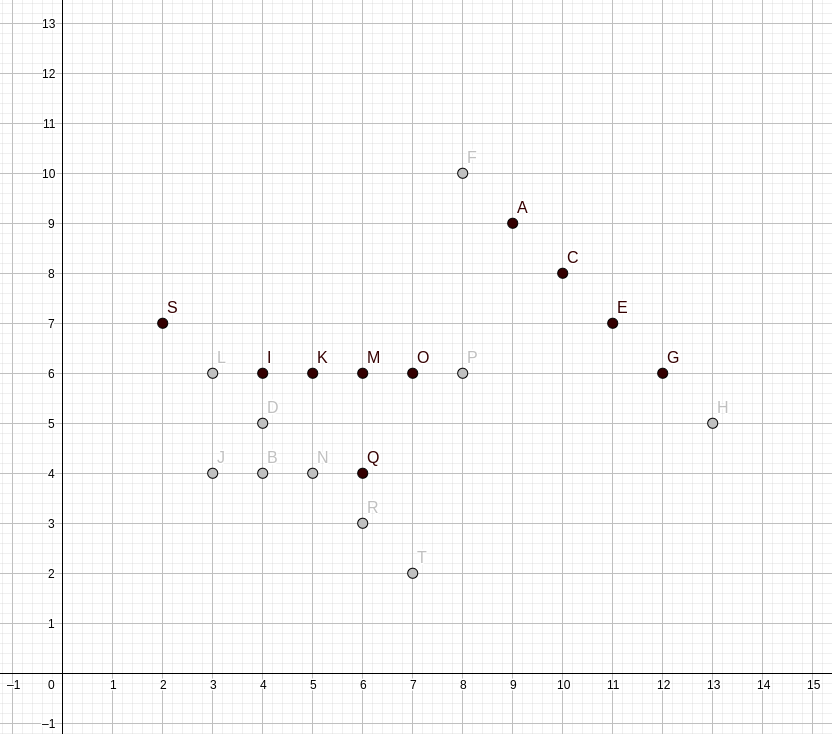
\includegraphics[width=1\textwidth]{2.png}

	
	\end{frame}
	\begin{frame}
		\frametitle{例题2优化2}

对于任意一个点找到一条到已知连通块的链,然后依次加入这个已知连通块即可。要找到$p^k(u)$,类似优化1中的二分即可。
\end{frame}
	\begin{frame}
		\frametitle{例题5:整数\footnote{集训队互测2021,作者:孙嘉伟}}
	
		
	

		交互库有排列$p:[0,n)\rightarrow[0,n)$,并内置了一个整数$I$,你可以询问$Q(i)$,交互库会将$I$加上$2^{p_i}$,并返回$I$中$1$的个数,最终你需要找出交互库的排列。

		\onslide<2->

		如果将每一个数都与恰好比它小$1$的数相连,这一道题的目的可以看做是找到一条链。

		连续的询问$Q(i),Q(i)$可以知道$I$的$2^{p_i}$位是否为$1$,并将$2^{p_i+1}$位变为$1$,随机排列$q$,询问$Q(q_i),Q(q_i)$,每次可以以$\dfrac 12$的概率去掉一个数$u$错误的前驱$v$,在$C\log n$次即可以将所有数所有错误的前驱去掉,最后只剩下它正确的那一个前驱,依次链接就成了答案对应的链。

		最后需要把$I$的前$n$为变为$0$,加上$2\times 2^0$即可,寻找$0$的位置可以通过$Q(0),Q(1)\dots,Q(n-1),Q(0),Q(1)\dots,Q(n-1)$做到。

	\end{frame}
	\begin{frame}
		\frametitle{交互库寄存器的处理}
	
		交互库有时还存在一个寄存器(如例题5),所以连续两次相同的询问可能会出现不同的答案,这会对分析造成极大的影响。

		一开始交互库寄存器的信息往往可以认为是毫无规律的,在经过若干操作时会变得有部分良好的性质,在通过分析返回值得到这些性质时,可以想着怎么去操作使得他们能够保留下来。

		更进一步,当寄存器的部分内容是自行选择写入时,对每一个写入元素代表状态明确区分有利于后面操作的分析。

		可以说,这一类题目最最重要的就是对未知的寄存器的把控。
	
	\end{frame}
	\begin{frame}
		\frametitle{例题6:Indiana Jones and the Uniform Cave\footnote{2016-2017 ACM-ICPC Northeastern European Regional Contest (NEERC 16)}}

		你现在在一个洞穴里。这个洞穴有 $n$ 个房间。房间是不可区分的。每个房间都引出 $m$ 个单向道路,终点可以是自己也可以是其它房间。这些单向道路的入口均匀地分布在房间的墙壁上,且每条单向道路也是不可区分的。保证整个有向图是强连通的。
		
		每个房间有一个石子,这也是你区分房间和道路的唯一工具。一开始石子是在这个房间的某一个通道的入口前,并且是放在中央的。你每到一个房间,可以选择将石子移动到某个通道前,把它放在通道左边或者右边(不能是中间),然后再从某个通道走出去。你不可以把石子带出房间。你一开始在某一个房间,你的目的是便利这个洞穴的所有边。
	\end{frame}
		
	\begin{frame}
		\frametitle{例题6}
		
		这道题的寄存器就是石头,一开始石头的摆放是很有规律的:全在中间,可以认为这就是良好的状态,自然的想法就是后续操作也以一定规律摆放石头,这样就可以方便把控寄存器的内容。
		
		因为石头是唯一一个提供的信息,不妨把一个的的出边认为是石头所在的边上,并且我们希望从一个点走出后可以回到这一个点上,所以不妨尽可能的让所有已知的节点和他们的出边组成一个内向森林,据此可以对石头的位置进行明确分类:
		
		\begin{itemize}
			\item 中间:第一次经过。
			\item 左边:确定的边。
			\item 右边:不能确定到哪的边。
		\end{itemize}
		
		右边会形成一条链,表示这些链上的点还没有找出所有的边。而沿左边最终都会到一个右边的点。
	\end{frame}
	\begin{frame}
		\frametitle{例题6}
		
			
		
		于是,这些石头就可以在已知的信息内指路,当确定一条边后,就继续尝试在顺时针的下一条边行走。当一个点的所有边都被走过,就恢复为左边,并放置将石头在能形成经过右边数量最多的环上。最后走到右链的末端。
		
		下面就是一个实例,加粗表示当前节点,1表示左边0表示右边,-1表示这条边上不放石头,为了使图示更美观,部分边被省略。

		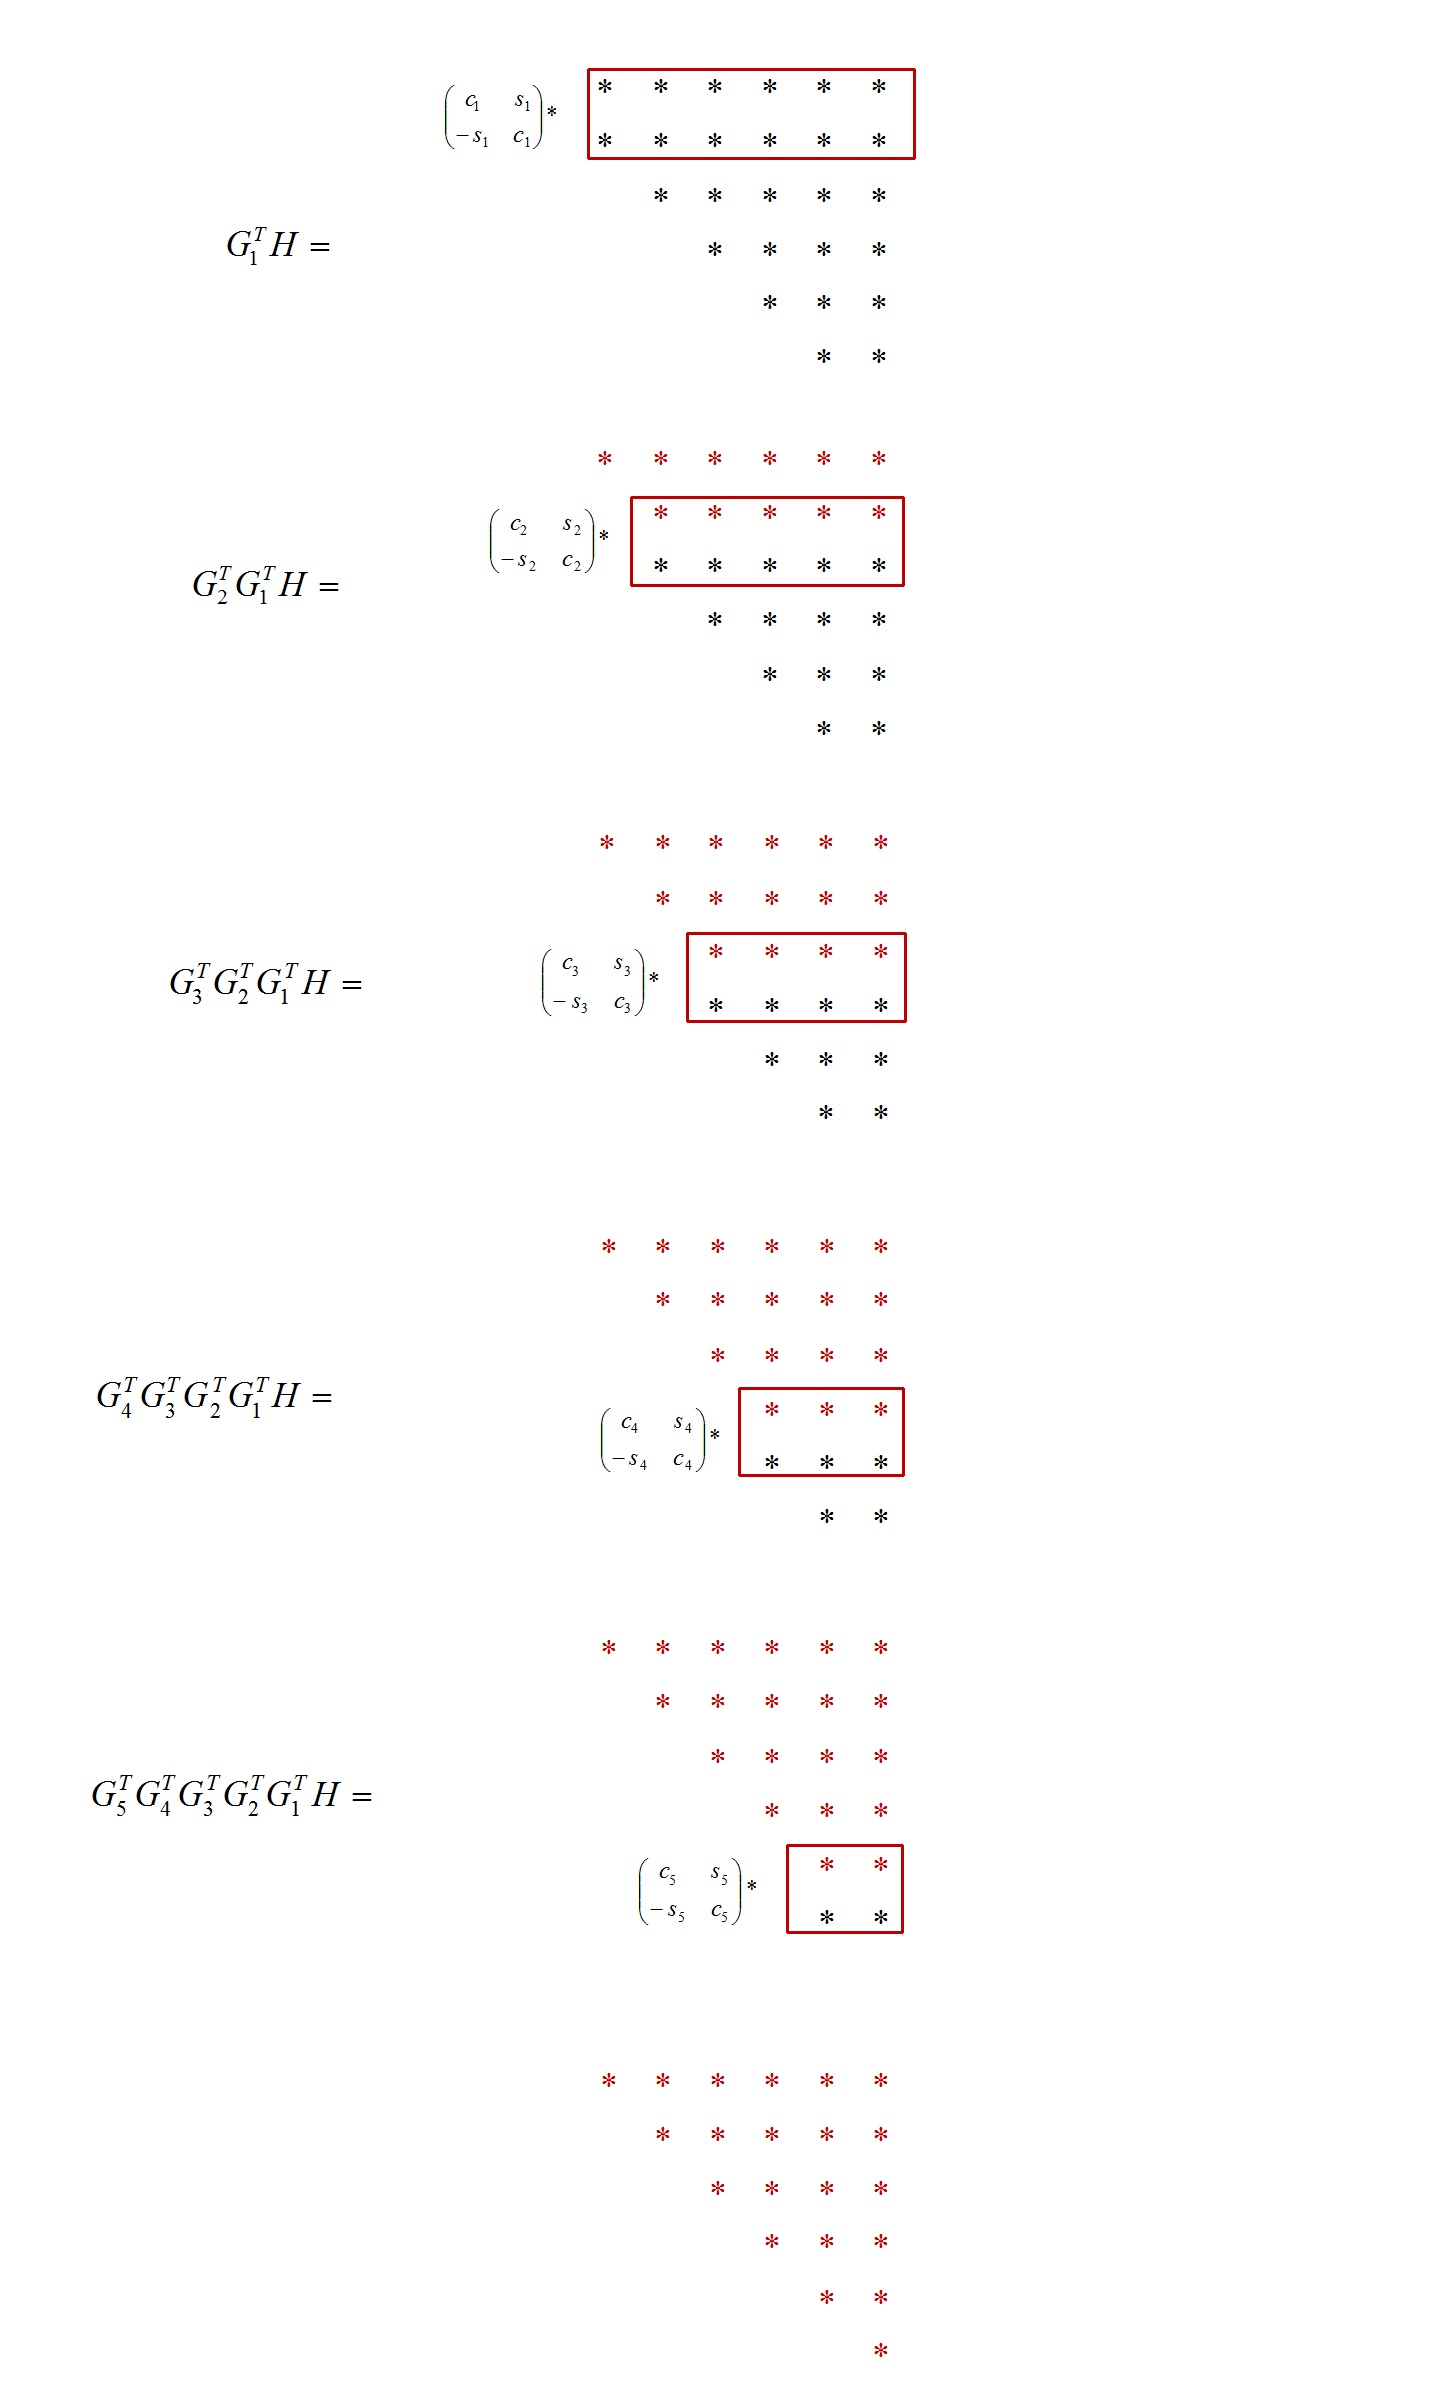
\includegraphics[width=0.24\textwidth]{6.png}
		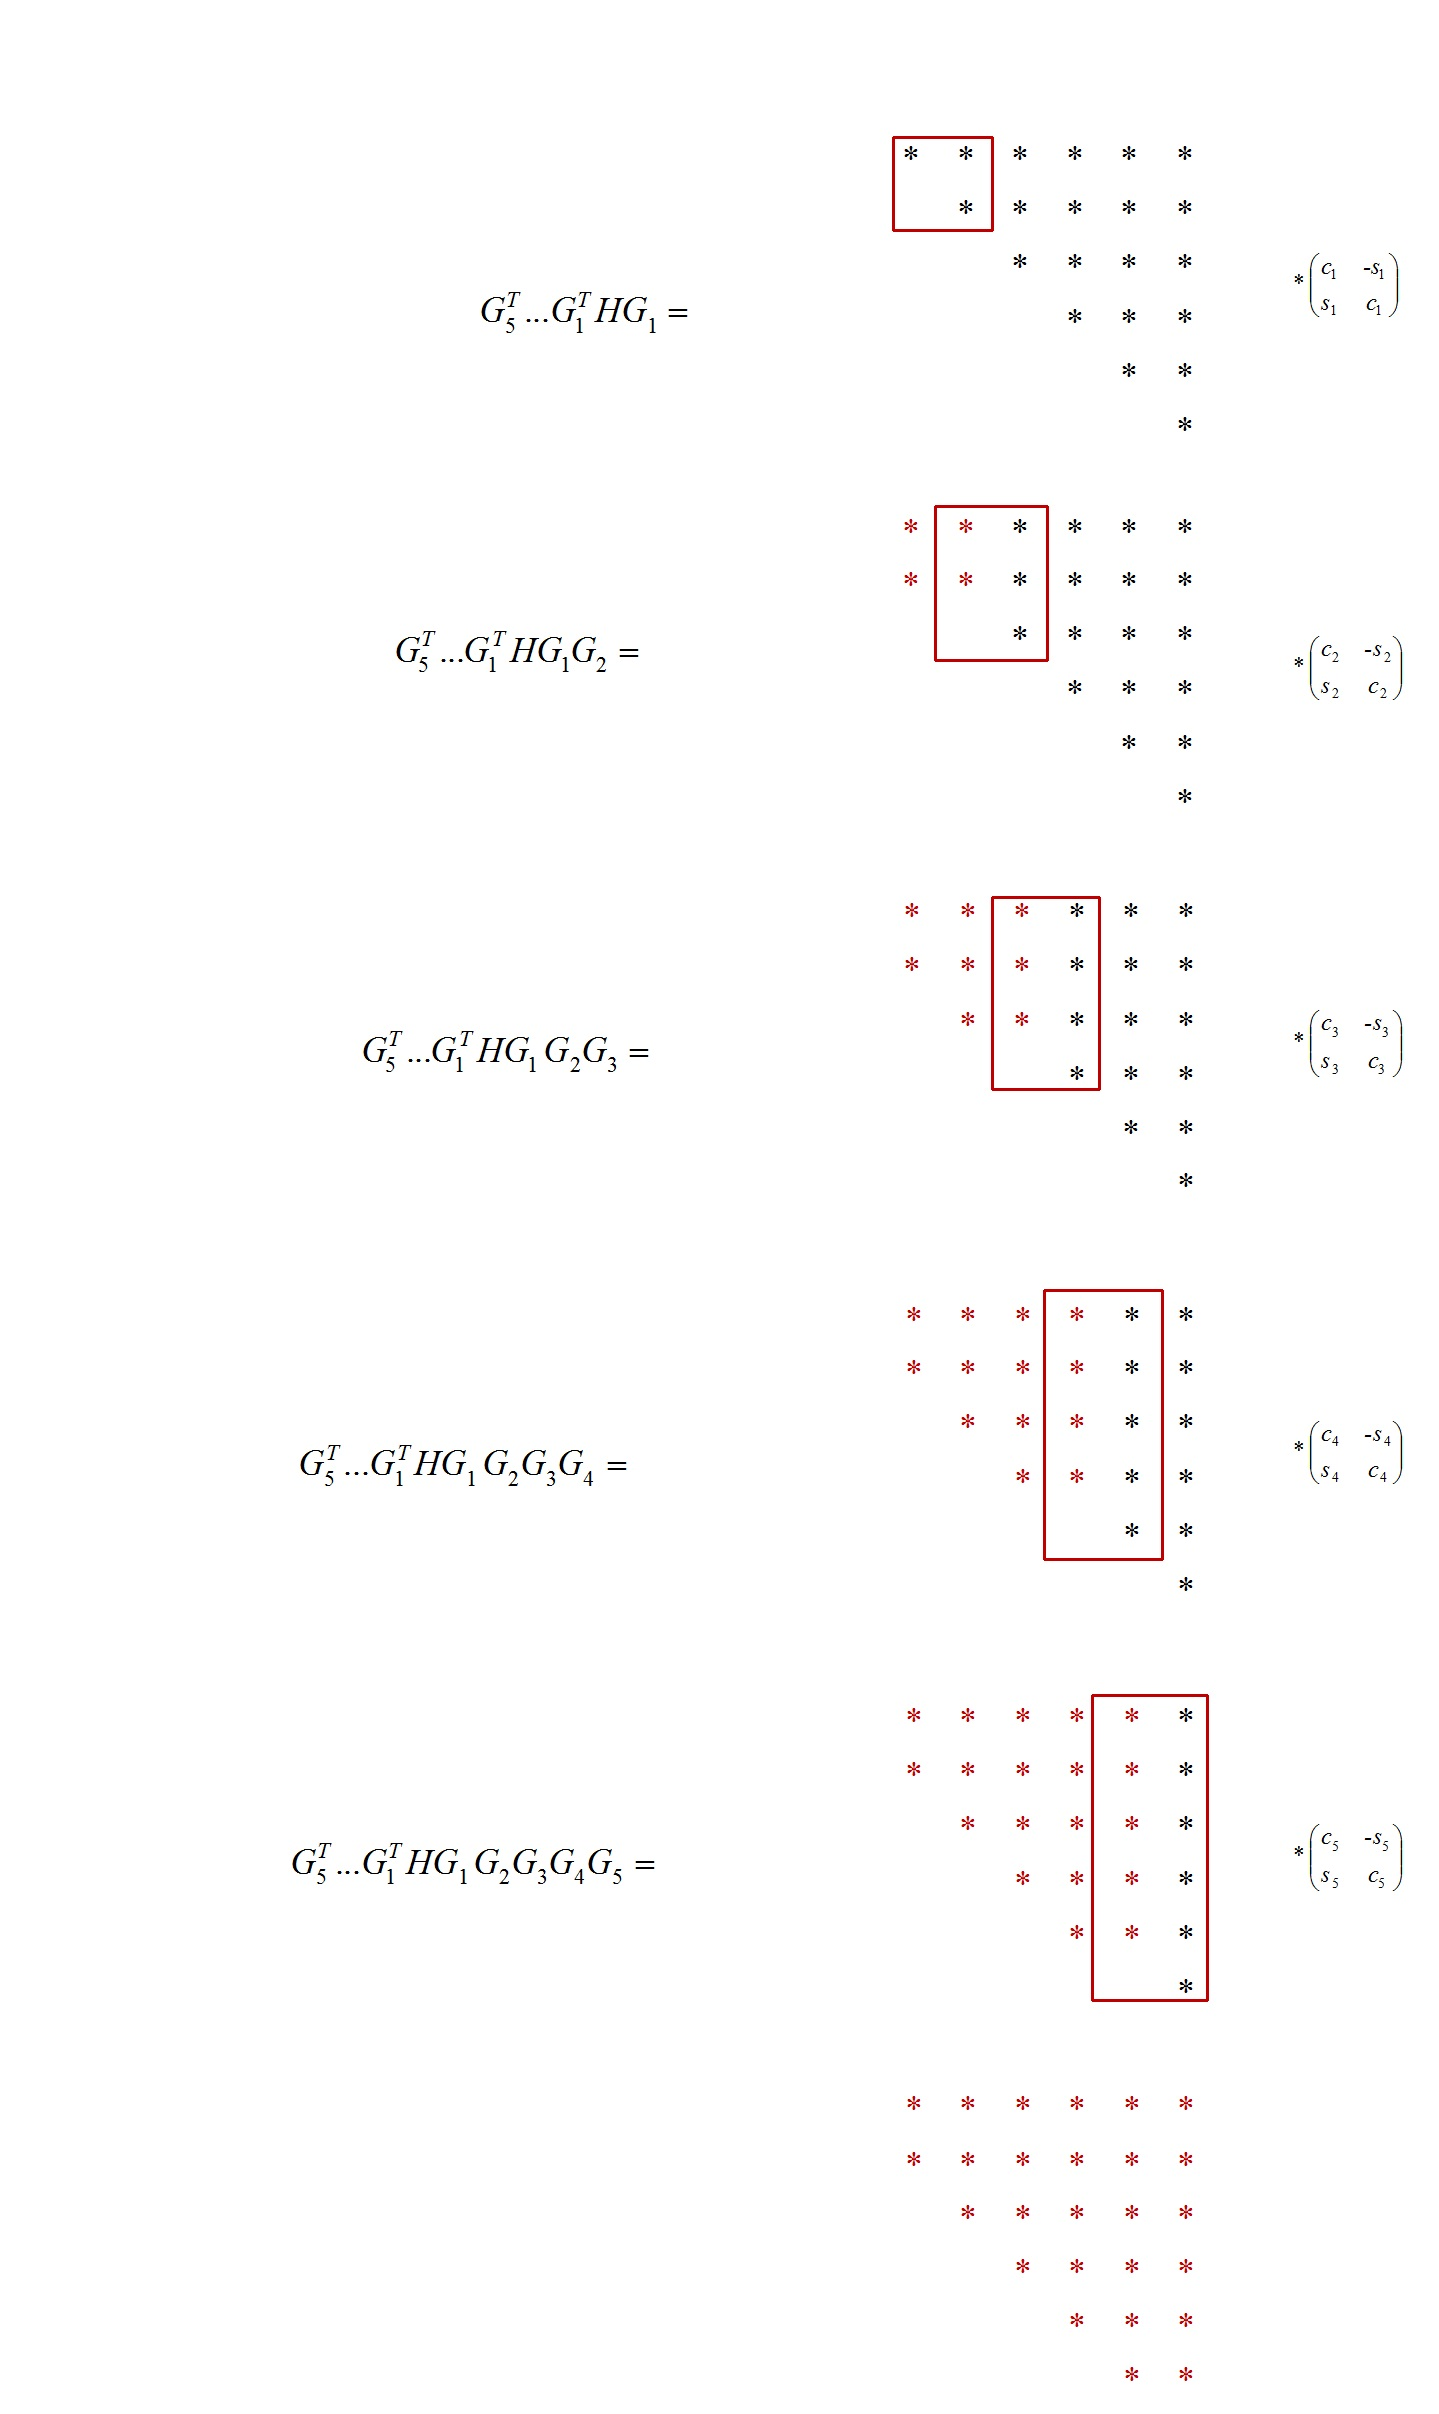
\includegraphics[width=0.24\textwidth]{7.png}
		\includegraphics[width=0.24\textwidth]{8.png}
		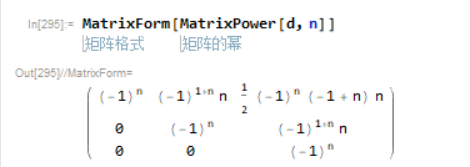
\includegraphics[width=0.24\textwidth]{5.png}
	
	\end{frame}
	\begin{frame}
		\frametitle{例题7: Rotary Laser Lock\footnote{codeforces 1428 H}}

		你有一个锁叫做旋转激光锁:
		
		\begin{itemize}
			\item 锁由编号为 $0$ 到 $n-1$ 的 $n$ 个同心环组成。最里面的环是环 $0$,最外面的环是环 $n-1$。
			\item 锁平均分成了 $n\times m$ 部分。每一个环都包含一个圆弧,正好覆盖了 $m$ 个相邻的部分(不同的若干个环可以覆盖同一段圆弧)。
			\item 你每次可以转动一个环一部分的长度,此时交互库会返回锁有多少个部分没有被任何圆环覆盖。
		\end{itemize}
		
		你需要通过若干次转动来得到与输出每一个圆环的当前位置。
		
		
	
	\end{frame}
	\begin{frame}
		\frametitle{例题7}
	
		对所有圆环依次执行:旋转一周,找到返回的最大值,然后旋转至返回值最大时位置最大处。

		这样就一定可以让所有圆环都有另一圆环与它重合。这就是一个非常好的性质。

		然后将所有重叠的圆环视作一个,这样就不会破坏那个性质了,重复上述过程,最终在$\log$次内停止。

	
	\end{frame}
\end{document}